%\renewcommand{\theequation}{\theenumi}
\begin{enumerate}[label=\thesection.\arabic*.,ref=\thesection.\theenumi]
\numberwithin{equation}{enumi}

\item Amongst all open (from the top) right circular cylindrical boxes of volume $125 \pi $ $cm^3$, find the dimensions of the box which has the least surface area.\\  
\solution Let $r$ be the radius of the cylinder and $h$ be the height.  Then the surface area is 
		\begin{align}
			\label{eq:opt-box-S}
			S &= \pi r^2 + 2\pi r h 
		\end{align}
		Also, the volume is 
		\begin{align}
			\label{eq:opt-box-V}
			V &= \pi r^2 h 
		\end{align}
			\item 
		The given problem can then be formulated as 
		\begin{align}
			S = \min_{r,h}\pi r^2 + 2\pi r h 
			\\
			\text{s.t} \quad \pi r^2 h =125 
		\end{align}
				which is a {\em disciplined geometric programming} (DGP) problem that can be solved using $cvxpy$. DGP is a subset of 
				 {\em log-log-convex program} (LLCP). An LLCP is defined as
				\begin{equation}
\begin{split}
\begin{array}{ll}
\mbox{minimize} & f_0(x) \\
\mbox{subject to} & f_i(x) \leq \tilde{f_i}, \quad i=1, \ldots, m\\
& g_i(x) = \tilde{g_i}, \quad i=1, \ldots, p,
\end{array}
\end{split}
\end{equation}
where the functions $f_i$
				are log-log convex, $\tilde{f}_i$
 are log-log concave, and the functions $g_i$
				and $\tilde{g}_i$
 are log-log affine. An optimization problem with constraints of the above form in which the goal is to maximize a log-log concave function is also an LLCP.
A function 
				\begin{align}
 f : D \subseteq \mathbf{R}^{n}_{++} \to \mathbf{R}
				\end{align}
				is said to be log-log convex if the function
				\begin{align}
				F(u)=\log f(e^u)
				\end{align}
				with domain
				\begin{align}
				\{u \in \mathbf{R}^n : e^u \in D\}
				\end{align}
				is convex (where
$				\mathbf{R}^{n}_{++}$
				denotes the set of positive reals and the logarithm and exponential are meant elementwise); the function $F$  is called the log-log transformation of $f$. The function $f$ is log-log concave if $F$ is concave, and it is log-log affine if $F$ is affine.
				LLCPs are problems that become convex after the variables, objective functions, and constraint functions are replaced with their logs, an operation that we refer to as a log-log transformation. LLCPs generalize geometric programming.
	\item 
		Alternatively, from 
			\eqref{eq:opt-box-S} and 
			\eqref{eq:opt-box-V}
		\begin{align}
			S(r) &= \pi r^2 +  \frac{2 V}{r} 
			\\
			\label{eq:opt-box-Sdiff}
			\implies 
			S^{\prime}(r) &= 2\pi r -  \frac{2 V}{r^2} 
			\\
			\text{and }
			S^{\prime\prime}(r) &= 2\pi  +  \frac{4 V}{r^3} > 0 
		\end{align}
		Thus, $S(r)$ has a minimum which can be obtained from 
			\eqref{eq:opt-box-Sdiff} as
		\begin{align}
			2\pi r -  \frac{2 V}{r^2} &= 0
			\\
			\implies r &= \brak{\frac{V}{\pi}}^{\frac{1}{3}}
			\\
			&= 5 \quad \text{and }
			\\
			h &= \frac{V}{\pi r^2} = 5
		\end{align}
		upon substituting numerical values.
		This is verified in 
Fig. 
	\ref{fig:opt-12-3}.
\begin{figure}[!h]
	\centering
	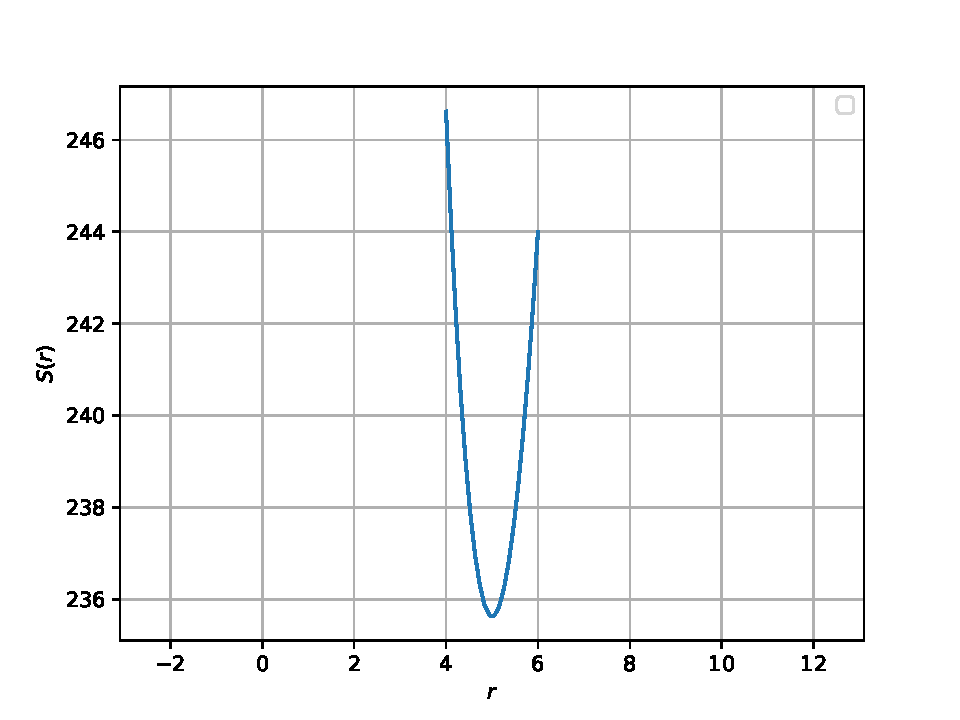
\includegraphics[width=\columnwidth]{figs/opt/opt-12-3.pdf}
	\caption{}
	\label{fig:opt-12-3}
\end{figure}
	\item Using gradient descent, the update equation can be expressed as 
		\begin{align}
			r_{n+1} &= r_n - \gamma S^{\prime}(r_n)
		\end{align}
		where $r_0 = 2$ and $\gamma = 0.001$ are chosen by the user.  These values need to be suitably guessed for the algorithm to converge.
\end{enumerate}


